\chapter{非平衡载流子}

\section{非平衡载流子的注入和复合}

处于热平衡下的载流子浓度称为\textbf{平衡载流子浓度}。一般用$n_0$和$p_0$分别表示平衡电子浓度和空穴浓度。非简并条件下,其乘积满足关系:
\begin{equation}
    n_0p_0=N_vN_c\exp{\left(-\frac{E_g}{k_0T}\right)}=n_i^2
\end{equation}

对半导体施加外界作用,破坏热平衡条件,使半导体处于与热平衡偏离的状态,称为\textbf{非平衡状态}。处于非平衡状态的半导体,其载流子浓度浓度不再为$n_0$和$p_0$,而会多出一部分。比平衡状态多出的载流子称为\textbf{非平衡载流子}或\textbf{过剩载流子}。

一定温度下,n型半导体中,$n_0\gg p_0$,用适当波长的光照射半导体,且光子能量大于半导体的禁带宽度,则光子可以将价带电子激发到导带上,形成电子-空穴对,导带比平衡时多出$\Delta n$的电子,即\textbf{非平衡电子},称为\textbf{非平衡多数载流子(多子)};价带多出$\Delta p$的空穴,即\textbf{非平衡空穴},称为\textbf{非平衡少数载流子(少子)}。这种通过光照产生非平衡载流子的方法,称为非平衡载流子的\textbf{光注入}。光注入时有:
\begin{equation}
    \Delta n=\Delta p
\end{equation}

一般情况下,注入的非平衡载流子浓度比平衡时的多数载流子浓度小得多。对上述情况,有:
\begin{equation}
    \Delta n\ll n_0,\quad \Delta p\ll n_0
\end{equation}
满足此条件的注入称为\textbf{小注入}。在小注入条件下,非平衡少子的浓度也可以比平衡少子的浓度大得多,如上例中有$\Delta p\gg p_0$。非平衡少子常常会起决定性作用。通常所说的非平衡载流子都指非平衡少子。

光注入导致半导体的电导率增大。附加电导率为:
\begin{equation}
    \Delta \sigma=\Delta nq\mu_n+\Delta pq\mu_p=\Delta pq(\mu_n+\mu_p)
\end{equation}

设半导体平衡电导率为$\sigma_0$,光照引起附加电导率$\Delta \sigma$,小注入条件下$\sigma_0+\Delta \sigma\approx\sigma_0$,电阻率改变:
\begin{equation}
    \Delta\rho=\frac{1}{\sigma}-\frac{1}{\sigma_0}=\frac{1}{\sigma_0+\Delta\sigma}-\frac{1}{\sigma_0}=-\frac{\Delta\sigma}{(\sigma_0+\Delta\sigma)\sigma_0}\approx-\frac{\Delta\sigma}{\sigma_0^2}
\end{equation}
半导体电阻改变:
\begin{equation}
    \Delta r=\Delta\rho\frac{l}{s}\approx-\frac{l}{s\sigma_0^2}\Delta\sigma
\end{equation}
$l,\ s$为半导体的长度和截面积。因此$\Delta r\propto \Delta \sigma$。半导体通电时,由于电势差$\Delta V=I\Delta r$,故$\Delta V\propto\Delta\sigma$,因此$\Delta V\propto\Delta p$:
\begin{equation}
    \Delta V=-\frac{l}{s\sigma^2}Iq(\mu_n+\mu_p)\Delta p
\end{equation}

\section{非平衡载流子的寿命}

小注入时,$\Delta V$的变化反映了$\Delta p$的变化。光照停止后,$\Delta p$随时间按指数减小。非平衡载流子的平均生存时间称为载流子的\textbf{寿命},用$\tau$表示(上章有个叫平均自由时间的物理量也记成$\tau$ 
\includegraphics[width=4em, align=c]{idiot.jpg})。由于非平衡少子相比多子更占主导地位,因此非平衡载流子的寿命常称为\textbf{少子的寿命}。显然$\D \frac{1}{\tau}$是单位时间内非平衡载流子的复合概率。\vspace{1ex}
通常将单位时间单位体积内净复合消失的电子-空穴对数称为非平衡载流子的\textbf{复合率}。显然,$\D \frac{\Delta p}{\tau}$就是复合率。

一束光在一块n型半导体内均匀产生非平衡载流子$\Delta n$和$\Delta p$。$t=0$时光照停止,\vspace{1ex}
$\Delta p$会随时间变化,单位时间内浓度减小$\D -\frac{\mathrm{d}\Delta p(t)}{\mathrm{d}t}$,减小是由电子-空穴对的复合引起的,应当等于非平衡载流子的复合率:
\begin{equation}
    \frac{\mathrm{d}\Delta p(t)}{\mathrm{d}t}=-\frac{\Delta p}{\tau}
\end{equation}
寿命$\tau$在小注入条件下是个恒量,与$\Delta p(t)$无关。解这个微分方程:
\begin{equation}
    \Delta p(t)=C\mathrm{e}^{-\frac{t}{\tau}}
\end{equation}
设$t=0$时刻停止光照时少子浓度$\Delta p(0)=\Delta p_0$,作为边界条件代入微分方程,解得系数为$C=\Delta p_0$,故:
\begin{equation}
    \Delta p(t)=\Delta p_0\mathrm{e}^{-\frac{t}{\tau}}
\end{equation}
即非平衡载流子浓度随时间按指数衰减。

\section{准费米能级}

热平衡下的半导体中电子和空穴具有统一的费米能级。非简并条件下:
\begin{equation}
    n_0=N_c\exp{\left(-\frac{E_c-E_F}{k_0T}\right)},\quad p_0=N_v\exp{\left(-\frac{E_F-E_v}{k_0T}\right)}\label{eq:chap-5-equilibrium-distribute}
\end{equation}
外界影响下破坏了热平衡,非平衡态的半导体不再具有统一的费米能级。我们认为价带和导带中的电子与空穴各自处于平衡状态,但价带与导带之间不处于平衡态。因此可以分别引入\textbf{导带费米能级}和\textbf{价带费米能级},均为\textbf{局部费米能级},称为\textbf{准费米能级}。导带费米能级也称为\textbf{电子准费米能级},用$E_{Fn}$表示,价带准费米能级也称为\textbf{空穴准费米能级},用$E_{Fp}$表示。

非平衡下的载流子浓度可以用与平衡载流子浓度类似公式表达:
\begin{equation}
    n=N_c\exp{\left(-\frac{E_c-E_{Fn}}{k_0T}\right)},\quad p=N_v\exp{\left(-\frac{E_{Fp}-E_v}{k_0T}\right)}
\end{equation}
上式适用的条件与平衡态载流子相同,即$E_{Fn}$和$E_{Fp}$不能进入导带或价带。参考\autoref{eq:chap-5-equilibrium-distribute},可以推导出$n$与$n_0$,$p$与$p_0$的关系:
\begin{align}
&
\begin{aligned}
    n&=N_c\exp{\left(-\frac{E_c-E_{Fn}}{k_0T}\right)}\\
    &=N_c\exp{\left(-\frac{E_c-E_{F}}{k_0T}\right)}\exp{\left(\frac{E_{Fn}-E_F}{k_0T}\right)}\\
    &=n_0\exp{\left(\frac{E_{Fn}-E_F}{k_0T}\right)}
\end{aligned}
\\
&
\begin{aligned}
    p&=N_v\exp{\left(-\frac{E_{Fp}-E_v}{k_0T}\right)}\\
    &=N_v\exp{\left(-\frac{E_{F}-E_v}{k_0T}\right)}\exp{\left(\frac{E_F-E_{Fp}}{k_0T}\right)}\\
    &=p_0\exp{\left(\frac{E_F-E_{Fp}}{k_0T}\right)}
\end{aligned}
\end{align}
由
\begin{equation}
    n_0=n_i\exp{\left(-\frac{E_i-E_F}{k_0T}\right)},\quad p_0=n_i\exp{\left(\frac{E_i-E_F}{k_0T}\right)}
\end{equation}
进一步推导:
\begin{align}
&
    \begin{aligned}
        n&=n_0\exp{\left(\frac{E_{Fn}-E_F}{k_0T}\right)}\\
        &=n_i\exp{\left(-\frac{E_i-E_F}{k_0T}\right)}\exp{\left(\frac{E_{Fn}-E_F}{k_0T}\right)}\\
        &=n_i\exp{\left(\frac{E_{Fn}-E_i}{k_0T}\right)}
    \end{aligned}
    \\
&
    \begin{aligned}
        p&=p_0\exp{\left(\frac{E_F-E_{Fp}}{k_0T}\right)}\\
        &=n_i\exp{\left(\frac{E_i-E_F}{k_0T}\right)}\exp{\left(\frac{E_F-E_{Fp}}{k_0T}\right)}\\
        &=n_i\exp{\left(\frac{E_i-E_{Fp}}{k_0T}\right)}
    \end{aligned}
\end{align}
电子与空穴浓度的乘积:
\begin{equation}
    np=n_0p_0\exp{\left(\frac{E_{Fn}-E_{Fp}}{k_0T}\right)}
\end{equation}

\section{复合理论}

\subsection{载流子复合的分类}

半导体\textbf{复合}的过程即半导体\textbf{由非平衡态向平衡态过渡}的过程。半导体的复合过程大致可分为:
\begin{enumerate}
    \item 直接复合:电子在导带与价带间直接跃迁,实现电子与空穴的复合。
    \item 间接复合:电子与空穴通过禁带能级复合。简介复合按照发生位置可以分为\textbf{体内复合}和\textbf{表面复合}。
\end{enumerate}
载流子复合时会放出多余能量,放出能量的方法有:
\begin{enumerate}
    \item 发射光子:伴随复合,伴有发光现象,称为\textbf{发光复合}或\textbf{辐射复合}。
    \item 发射声子:载流子将多余能量传递给晶格,加强晶格振动。
    \item 能量给予其他载流子,增大动能,称为\textbf{俄歇(Auger)复合}。
\end{enumerate}

\subsection{直接复合}

半导体中同时存在着载流子的\textbf{产生}和和\textbf{复合}两个过程。单位时间内产生的电子-空穴对数称为\textbf{产生率},记为$G$,复合的电子-空穴对数称为\textbf{复合率},记为$R$。

$n,\ p$分别为电子和空穴浓度。单位体积,单位时间里,每个电子都有概率和空穴复合,复合概率与空穴浓度成正比,即每个电子复合的概率为$rp$,$r$是比例系数。每个电子复合概率再乘以电子浓度就是全部电子的复合率,即:
\begin{equation}
    R=rnp
\end{equation}
比例系数$r$称为\textbf{电子-空穴复合概率},它代表着所有电子和空穴复合概率的平均值。

载流子受激发的概率不受载流子浓度的影响,产生率在所有非简并情况下是相同的,即$G$仅与温度有关,和$n,\ p$无关。

热平衡时,产生率等于复合率:$P=G$,此时$n=n_0,\ p=p_0$,因此得到$G$与$r$的关系:
\begin{equation}
    G=P=rn_0p_0=rn_i^2
\end{equation}
复合率减产生率即非平衡载流子的净复合率,得到净复合率$U_d$为:
\begin{equation}
    U_d=R-G=rnp-rn_i^2=r(np-n_i^2)
\end{equation}
代入关系$n=n_0+\Delta n,\ p=p_0+\Delta p,\ \Delta n=\Delta p$,得:
\begin{align}
    U_d&=r[(n_0+\Delta n)(p_0+\Delta p)-n_0p_0]\notag\\
    &=r(n_0\Delta p+p_0\Delta p+\Delta p^2)\notag\\
    &=r(n_0+p_0)\Delta p+r\Delta p^2
\end{align}
由于净复合率和载流子寿命存在关系:
\begin{equation}
    U_d=\frac{\Delta p}{\tau}
\end{equation}
得载流子寿命:
\begin{equation}
    \tau=\frac{\Delta p}{U_d}=\frac{1}{r[(n_0+p_0)+\Delta p]}\label{eq:chap-5-direct-recombination-lifetime}
\end{equation}
可见寿命$\tau$不仅与平衡载流子浓度有关,也与非平衡载流子浓度有关。

在小注入条件下,$\Delta p\ll (n_0+p_0)$,\autoref{eq:chap-5-direct-recombination-lifetime}近似为:
\begin{equation}
    \tau\approx\frac{1}{r(n_0+p_0)}
\end{equation}
对n型材料,$n_0\gg p_0$,上式近似有
\begin{equation}
    \tau\approx\frac{1}{rn_0}
\end{equation}
寿命与非平衡载流子无关,与多数载流子成反比。

当$\Delta p\gg n_0+p_0$时,\autoref{eq:chap-5-direct-recombination-lifetime}近似有:
\begin{equation}
    \tau\approx\frac{1}{r\Delta p}
\end{equation}
此时寿命与非平衡载流子成反比。

\subsection{间接复合}

半导体中的杂质和缺陷会促进非平衡载流子的复合过程,这些促进复合的杂质和缺陷称为\textbf{复合中心}。间接复合即非平衡载流子通过复合中心的复合。

记复合中心能级$E_t$,如\autoref{fig:indirect-recombination-process},能级$E_t$上的间接复合具有四个过程:
\begin{enumerate}[(1)]
    \item 俘获电子:复合中心能级$E_t$从导带俘获电子。
    \item 发射电子:复合中心能级$E_t$上的电子被激发到导带。
    \item 俘获空穴:电子由复合中心能级$E_t$落入价带,与空穴复合,可以看成复合中心能级$E_t$从价带俘获一个电子。
    \item 发射空穴:价带电子激发到复合中心能级$E_t$,可以看出复合中心能级$E_t$向价带发射一个空穴。
\end{enumerate}

\begin{figure}[ht]
    \centering
\tikzset{every picture/.style={line width=0.75pt}} %set default line width to 0.75pt        

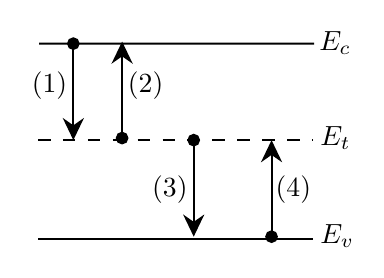
\begin{tikzpicture}[x=0.75pt,y=0.75pt,yscale=-1,xscale=1]
%uncomment if require: \path (0,300); %set diagram left start at 0, and has height of 300

%Straight Lines [id:da20064609469527683] 
\draw    (120.67,31.08) -- (137.17,31.09) -- (253.17,31.1) ;
%Straight Lines [id:da19330925404980026] 
\draw  [dash pattern={on 4.5pt off 4.5pt}]  (120.17,77.5) -- (252.67,77.5) ;
%Straight Lines [id:da5528060898844296] 
\draw    (120.17,125) -- (252.67,125) ;
%Shape: Circle [id:dp32843318610089023] 
\draw  [fill={rgb, 255:red, 0; green, 0; blue, 0 }  ,fill opacity=1 ] (134.63,31.09) .. controls (134.63,32.49) and (135.76,33.63) .. (137.17,33.63) .. controls (138.57,33.63) and (139.71,32.49) .. (139.71,31.09) .. controls (139.71,29.68) and (138.57,28.54) .. (137.17,28.54) .. controls (135.76,28.54) and (134.63,29.68) .. (134.63,31.09) -- cycle ;
%Straight Lines [id:da48904866335535435] 
\draw    (137.17,31.09) -- (137.17,74.58) ;
\draw [shift={(137.17,77.58)}, rotate = 270] [fill={rgb, 255:red, 0; green, 0; blue, 0 }  ][line width=0.08]  [draw opacity=0] (10.72,-5.15) -- (0,0) -- (10.72,5.15) -- (7.12,0) -- cycle    ;
%Straight Lines [id:da7345813081514647] 
\draw    (160.67,33.09) -- (160.67,76.58) ;
\draw [shift={(160.67,30.09)}, rotate = 90] [fill={rgb, 255:red, 0; green, 0; blue, 0 }  ][line width=0.08]  [draw opacity=0] (10.72,-5.15) -- (0,0) -- (10.72,5.15) -- (7.12,0) -- cycle    ;
%Shape: Circle [id:dp42146991706121617] 
\draw  [fill={rgb, 255:red, 0; green, 0; blue, 0 }  ,fill opacity=1 ] (158.12,76.58) .. controls (158.12,77.99) and (159.26,79.13) .. (160.67,79.13) .. controls (162.07,79.13) and (163.21,77.99) .. (163.21,76.58) .. controls (163.21,75.18) and (162.07,74.04) .. (160.67,74.04) .. controls (159.26,74.04) and (158.12,75.18) .. (158.12,76.58) -- cycle ;
%Straight Lines [id:da21853964923058133] 
\draw    (195.17,77.59) -- (195.17,121.08) ;
\draw [shift={(195.17,124.08)}, rotate = 270] [fill={rgb, 255:red, 0; green, 0; blue, 0 }  ][line width=0.08]  [draw opacity=0] (10.72,-5.15) -- (0,0) -- (10.72,5.15) -- (7.12,0) -- cycle    ;
%Shape: Circle [id:dp8914894742891817] 
\draw  [fill={rgb, 255:red, 0; green, 0; blue, 0 }  ,fill opacity=1 ] (192.63,77.59) .. controls (192.63,78.99) and (193.76,80.13) .. (195.17,80.13) .. controls (196.57,80.13) and (197.71,78.99) .. (197.71,77.59) .. controls (197.71,76.18) and (196.57,75.04) .. (195.17,75.04) .. controls (193.76,75.04) and (192.63,76.18) .. (192.63,77.59) -- cycle ;
%Straight Lines [id:da2456794806958813] 
\draw    (232.67,80.59) -- (232.67,124.08) ;
\draw [shift={(232.67,77.59)}, rotate = 90] [fill={rgb, 255:red, 0; green, 0; blue, 0 }  ][line width=0.08]  [draw opacity=0] (10.72,-5.15) -- (0,0) -- (10.72,5.15) -- (7.12,0) -- cycle    ;
%Shape: Circle [id:dp5273521015953397] 
\draw  [fill={rgb, 255:red, 0; green, 0; blue, 0 }  ,fill opacity=1 ] (230.12,124.08) .. controls (230.12,125.49) and (231.26,126.63) .. (232.67,126.63) .. controls (234.07,126.63) and (235.21,125.49) .. (235.21,124.08) .. controls (235.21,122.68) and (234.07,121.54) .. (232.67,121.54) .. controls (231.26,121.54) and (230.12,122.68) .. (230.12,124.08) -- cycle ;

% Text Node
\draw (115.67,43) node [anchor=north west][inner sep=0.75pt]   [align=left] {(1)};
% Text Node
\draw (162,43) node [anchor=north west][inner sep=0.75pt]   [align=left] {(2)};
% Text Node
\draw (173.67,93) node [anchor=north west][inner sep=0.75pt]   [align=left] {(3)};
% Text Node
\draw (233.17,93) node [anchor=north west][inner sep=0.75pt]   [align=left] {(4)};
% Text Node
\draw (254.67,116.9) node [anchor=north west][inner sep=0.75pt]    {$E_{v}$};
% Text Node
\draw (254.17,23.9) node [anchor=north west][inner sep=0.75pt]    {$E_{c}$};
% Text Node
\draw (254.67,69.4) node [anchor=north west][inner sep=0.75pt]    {$E_{t}$};
\end{tikzpicture}
    \caption{复合中心能级$E_t$的四个间接复合过程}
    \label{fig:indirect-recombination-process}
\end{figure}

$n$和$p$分别为导带电子和价带空穴浓度,设复合中心浓度为$N_t$,复合中心能级上的电子浓度为$n_t$,则未被电子占据的复合中心浓度为$N_t-n_t$。

(1) 过程中,我们把单位体积、单位时间内内复合中心俘获的电子数称为\textbf{电子俘获率}。电子俘获率与导带电子浓度$n$和未被占据的复合中心浓度$(N_t-n_t)$成正比:
\begin{equation}
    \text{电子俘获率}=r_nn(N_t-n_t)\label{eq:chap-5-indirect-recombination-electron-capture-rate}
\end{equation}
比例系数$r_n$是\textbf{电子俘获系数},反映了复合中心平均俘获电子能力的大小。

(2) 过程是 (1) 过程的逆过程。我们用电子产生率表示单位时间、单位体积向导带发射的电子数。只有已被占据的复合中心才能向导带发射电子,导带近似认为是空的,因此电子产生率与$n_t$成正比,和$n$无关:
\begin{equation}
    \text{电子产生率}=s_-n_t
\end{equation}
$s_-$称为\textbf{电子激发概率},仅与温度有关。

平衡时,(1) 过程和 (2) 过程相互抵消,电子产生率等于电子俘获率:
\begin{equation}
    r_nn_0(N_t-n_{t0})=s_-n_{t0}\label{eq:chap-5-equilibrium-indirect-recombination-electron-equation}
\end{equation}
$n_0$和$n_{t0}$分别为平衡时导带和复合中心能级上的电子浓度。计算$n_{t0}$时,我们忽略分布函数中的简并因子:
\begin{equation}
    n_{t0}=N_tf(E_t)=N_t\frac{1}{\D 1+\exp{\left(\frac{E_t-E_F}{k_0T}\right)}}
\end{equation}
非简并条件下:
\begin{equation}
    n_0=N_c\exp{\left(\frac{E_F-E_c}{k_0T}\right)}
\end{equation}
将$n_0$和$n_{t0}$表达式代入\autoref{eq:chap-5-equilibrium-indirect-recombination-electron-equation}:
\begin{align}
    s_-N_t\frac{1}{\D 1+\exp{\left(\frac{E_t-E_F}{k_0T}\right)}}&=r_nN_c\exp{\left(\frac{E_F-E_c}{k_0T}\right)}N_t\left[1-\left(\frac{1}{\D 1+\exp{\left(\frac{E_t-E_F}{k_0T}\right)}}\right)\right]\notag\\
    \Longrightarrow s_-&=r_nN_c\exp{\left(\frac{E_F-E_c}{k_0T}\right)}\exp{\left(\frac{E_t-E_F}{k_0T}\right)}\notag\\
    \Longrightarrow s_-&=r_nN_c\exp{\left(\frac{E_t-E_c}{k_0T}\right)}
\end{align}
记:
\begin{equation}
    n_1=N_c\exp{\left(\frac{E_t-E_c}{k_0T}\right)}
\end{equation}
$n_1$等于费米能级与复合中心能级重合时导带电子平均浓度。代入:
\begin{equation}
    s_-=r_nN_c\exp{\left(\frac{E_t-E_c}{k_0T}\right)}=r_nn_1
\end{equation}
将上式代入电子产生率中:
\begin{equation}
    \text{电子产生率}=r_nn_1n_t\label{eq:chap-5-indirect-recombination-electron-generation-rate}
\end{equation}

(3) 过程中,空穴俘获率与$n_t$和$p$成正比:
\begin{equation}
    \text{空穴俘获率}=r_ppn_t\label{eq:chap-5-indirect-recombination-hole-capture-rate}
\end{equation}
$r_p$称为\textbf{空穴俘获系数},反映复合中心平均俘获空穴的能力.

(4) 过程是 (3) 的逆过程类似上文讨论,有:
\begin{equation}
    \text{空穴产生率}=s_+(N_t-n_t)
\end{equation}
$s_+$为\textbf{空穴激发概率}。

平衡时,(3) 和 (4) 过程相互抵消:
\begin{equation}
    s_+(N_t-n_{t0})=r_pp_0n_{t0}
\end{equation}
代入平衡时$p_0$和$n_{t0}$值,得:
\begin{equation}
    s_+=r_pp_1
\end{equation}
其中
\begin{equation}
    p_1=N_v\exp{\left(-\frac{E_t-E_v}{k_0T}\right)}
\end{equation}
$p_1$等于费米能级和复合中心能级重合时价带的平衡空穴浓度。

将$s_+$表达式代入空穴产生率,得:
\begin{equation}
    \text{空穴产生率}=r_pp_1(N_t-n_t)\label{eq:chap-5-indirect-recombination-hole-generation-rate}
\end{equation}
在稳定情况下,(1) 到 (4) 过程满足复合中心上电子数不变,即$n_t$为常数。由于 (1)  (4)两个过程造成复合中心上电子累积,(2) (3) 两个过程造成复合中心上电子的减少,为保持$n_t$不变,满足:
\begin{equation}
    \text{(1)}+\text{(4)}=\text{(2)}+\text{(3)}
\end{equation}
代入\autoref{eq:chap-5-indirect-recombination-electron-capture-rate}、\autoref{eq:chap-5-indirect-recombination-electron-generation-rate}、\autoref{eq:chap-5-indirect-recombination-hole-capture-rate}、\autoref{eq:chap-5-indirect-recombination-hole-generation-rate}:
\begin{equation}
    r_nn(N_t-n_t)+r_pp_1(N_t-n_t)=r_nn_1n_t+r_ppn_t\label{eq:chap-5-indirect-recombination-center-electron-conecntration-equation}
\end{equation}
求解$n_t$,得:
\begin{equation}
    n_t=N_t\frac{r_nn+r_pp_1}{r_n(n+n_1)+r_p(p+p_1)}\label{eq:chap-5-indirect-recombination-center-electron-conecntration}
\end{equation}

半导体的电子复合率为 $\text{(1)}-\text{(2)}$,空穴复合率为 $\text{(3)}-\text{(4)}$由于电子和空穴成对出现,二者应相等,等于半导体的净复合率$U_d$:
\begin{equation}
    U=\text{(1)}-\text{(2)}=\text{(3)}-\text{(4)}
\end{equation}
将\autoref{eq:chap-5-indirect-recombination-center-electron-conecntration-equation}代入上式:
\begin{equation}
    U=N_t\frac{r_nr_p\left(np-n_1p_1\right)}{r_n(n+n_1)+r_p(p+p_1)}\label{eq:chap-5-indirect-recombination-center-total-recombination-rate-1}
\end{equation}
由于:
\begin{equation}
    n_1=N_c\exp{\left(\frac{E_t-E_c}{k_0T}\right)},\quad p_1=N_v\exp{\left(-\frac{E_t-E_v}{k_0T}\right)}
\end{equation}
得到:
\begin{equation}
    n_1p_1=N_cN_v\exp{\left(\frac{E_v-E_c}{k_0T}\right)}=n_i^2
\end{equation}
代入\autoref{eq:chap-5-indirect-recombination-center-total-recombination-rate-1},得到非平衡载流子复合率:
\begin{equation}
    U=N_t\frac{r_nr_p\left(np-n_i^2\right)}{r_n(n+n_1)+r_p(p+p_1)}\label{eq:chap-5-indirect-recombination-center-charge-carrier-total-recombination-rate}
\end{equation}
上式即通过复合中心复合的净复合率一般公式。

热平衡条件下,$np=n_0p_0=n_i^2$,代入\autoref{eq:chap-5-indirect-recombination-center-charge-carrier-total-recombination-rate},显然有$U=0$。

对半导体注入非平衡载流子,有$np>n_i^2$,$U>0$。代入关系$n=n_0+\Delta n,\ p=p_0+\Delta p,\ \Delta n=\Delta p$:
\begin{equation}
    U=N_t\frac{r_nr_p\left(n_0\Delta p+p_0\Delta p+\Delta p^2\right)}{r_n\left(n_0+n_1+\Delta p\right)+r_p\left(p_0+p_1+\Delta p\right)}
\end{equation}
非平衡载流子的寿命为:
\begin{equation}
    \tau=\frac{\Delta p}{U}=\frac{r_n\left(n_0+n_1+\Delta p\right)+r_p\left(p_0+p_1+\Delta p\right)}{N_tr_nr_p(n_0+p_0+\Delta p)}
\end{equation}
寿命$\tau$和复合中心浓度$N_t$成反比。

在小注入条件下$\Delta p\ll (n_0+p_0)$,对于一般的复合中心,$r_n$和$r_p$相差不大,分子和分母上的$\Delta p$可以忽略:
\begin{equation}
    \tau=\frac{r_n(n_0+n_1)+r_p(p_0+p_1)}{N_tr_nr_p(n_0+p_0)}
\end{equation}
可见小注入条件下,寿命与非平衡载流子浓度无关。

对于n型半导体,假定复合中心能级$E_t$接近价带,并令$E_t$关于禁带中心对称的能级位置为$E_t'$,$E_F$比$E_t'$更接近$E_c$,此时称为\textbf{强n型区},满足$n_0\gg p_0,\ n_0\gg n_1,\ n_0\gg p_1$,寿命化为:
\begin{equation}
    \tau=\tau_p\approx\frac{1}{N_t\tau_p}\label{eq:chap-5-indirect-recombination-n-type-strong-n-lifetime}
\end{equation}
因此在重掺杂的n型半导体中,对寿命起决定性作用的是复合中心对少数载流子(空穴)的俘获系数$r_p$,与电子俘获系数$r_n$无关。

若$E_F$在$E_i$和$E_t'$之间,称为\textbf{高阻区}。此时$p_1\gg n_0,\ p_1\gg p_0,\ p_1\gg n_1$,同时$n_0\gg p_0$,寿命:
\begin{equation}
    \tau\approx\frac{p_1}{N_tr_n}\frac{1}{n_0}
\end{equation}
高阻区中的寿命与多子浓度成反比,即与电导率成反比。

对于p型材料,仍假定$E_t$接近价带,当$E_F$比$E_t$更接近$E_v$时,称为\textbf{强p型区},寿命为:
\begin{equation}
    \tau=\tau_n\approx\frac{1}{N_tr_n}\label{eq:chap-5-indirect-recombination-p-type-strong-p-lifetime}
\end{equation}
可见复合中心对少子的俘获决定寿命。对\textbf{高阻区},有:
\begin{equation}
    \tau\approx\frac{p_1}{N_tr_n}\frac{1}{p_0}
\end{equation}
\vspace{1ex}若复合中心更接近导带,则高阻区的寿命公式中$\D\frac{p_1}{r_n}$应当用$\D \frac{n_1}{r_p}$代替。

将强n区寿命\autoref{eq:chap-5-indirect-recombination-n-type-strong-n-lifetime}和强p区寿命\autoref{eq:chap-5-indirect-recombination-p-type-strong-p-lifetime}代入非平衡载流子复合率
\autoref{eq:chap-5-indirect-recombination-center-charge-carrier-total-recombination-rate},得:
\begin{align}
    U&=\frac{np-n_i^2}{\D \frac{1}{N_tr_p}(n+n_1)+\frac{1}{N_tr_n}(p+p_1)}\notag\\
    &=\frac{np-n_i^2}{\tau_p(n+n_1)+\tau_n(p+p_1)}
\end{align}
由于
\begin{equation}
    n_1=n_i\exp{\left(\frac{E_t-E_i}{k_0T}\right)},\quad p_1=n_i\exp{\left(\frac{E_i-E_t}{k_0T}\right)}
\end{equation}
代入:
\begin{equation}
    U=\frac{np-n_i^2}{\D \tau_p\left[n+n_i\exp{\left(\frac{E_t-E_i}{k_0T}\right)}\right]+\tau_n\left[p+n_i\exp{\left(\frac{E_i-E_t}{k_0T}\right)}\right]}\label{eq:chap-5-indirect-recombination-center-charge-carrier-total-recombination-rate-Ei-Et}
\end{equation}
\vspace{1ex}假定$r=r_n=r_p$,则$\D \tau_n=\tau_p=\frac{1}{N_tr}$,化简,得:
\begin{align}
    U&=\frac{N_tr\left(np-n_i^2\right)}{\D n+p+n_i\left[\exp{\left(\frac{E_t-E_i}{k_0T}\right)}+\exp{\left(-\frac{E_t-E_i}{k_0T}\right)}\right]}\notag\\
    &=\frac{N_tr\left(np-n_i^2\right)}{\D n+p+2n_i\cosh{\left(\frac{E_t-E_i}{k_0T}\right)}}
\end{align}
\vspace{1ex}可以看出,$E_t\approx E_i$时,$\D\cosh{\left(\frac{E_t-E_i}{k_0T}\right)}\rightarrow \cosh{(0)}=1$极小,$U$趋于极大。如Cu,Fe,Au等杂质在Si中形成深能级,是有效的复合中心。远离禁带中央的浅能级不能起到有效的复合中心作用。

我们假设复活中心是具有一定半径的球体,其截面为$\sigma$。截面积越大,载流子运动中被复合中心俘获概率越大。因此可以用$\sigma$表示复合中心俘获载流子的本领,称为\textbf{俘获截面}。复合中心俘获电子和空穴的本领不同,因此分别用\textbf{电子俘获截面}$\sigma_+$和\textbf{空穴俘获截面}$\sigma_-$来表示。

载流子热运动速度$v_T$越大,它被复合中心俘获的概率也就越大。按照统计力学计算,得到$\D v_T=\sqrt{\frac{3k_0T}{m^*}}$。
若不区分电子和空穴有效质量,$300\ \mathrm{K}$时,有$v_T=10^7\ \mathrm{cm/s}$。\vspace{1ex}

俘获截面与俘获系数的关系有:
\begin{equation}
    r_n=\sigma_-v_T,\quad r_p=\sigma_+v_T
\end{equation}
利用此关系,可将\autoref{eq:chap-5-indirect-recombination-center-charge-carrier-total-recombination-rate-Ei-Et}重写为:
\begin{equation}
    U=\frac{\sigma_+\sigma_-v_TN_t(np-n_i^2)}{\D \sigma_-\left[n+n_i\exp{\left(\frac{E_t-E_i}{k_0T}\right)}\right]+\sigma_+\left[p+n_i\exp{\left(\frac{E_i-E_t}{k_0T}\right)}\right]}
\end{equation}
实验表明,Mn,Fe,Co,Au,Cu,Ni可以在Ge中形成复合中心;Au,Cu,Fe,Mn,In可以在Si中形成复合中心。

\subsection{表面复合}

少子寿命很大程度上受半导体样品的形状和表面状态影响。\textbf{表面复合}指在半导体表面发生的复合过程。表面的杂质和缺陷在禁带形成复合中心能级,因此表面复合仍是间接复合。

实际测得的寿命是体内复合和表面复合的综合结果。设这两种复合同时地单独平行发生,\vspace{1ex}
记体内复合寿命为$\tau_v$,
\vspace{1ex}则$\D \frac{1}{\tau_v}$就是体内复合概率。记表面复合寿命为$\tau_s$,则$\D \frac{1}{\tau_s}$就是表面复合概率。总概率为:
\begin{equation}
    \frac{1}{\tau}=\frac{1}{\tau_v}+\frac{1}{\tau_s}
\end{equation}
$\tau$称为\textbf{有效寿命}。

把单位时间内通过单位表面积复合的电子-空穴对数称为\textbf{表面复合率},记$U_s$。表面复合率$U_s$与表面处非平衡载流子浓度$\Delta p_s$成正比:
\begin{equation}
    U_s=s\Delta p_s
\end{equation}
比例系数$s$表示表面复合的强弱,量纲为速度,称为\textbf{表面复合速度}。

\section{陷阱效应}

能级上的电子通过载流子的俘获和产生过程和载流子保持平衡。对于非平衡态的载流子,这种平衡会受到破坏。电子增加,说明能级有收容非平衡载流子的作用;电子减少,说明能级有收容空穴的作用。杂质能级积累非平衡载流子的作用称为\textbf{陷阱效应}。所有的杂质能级都有陷阱效应,我们只考虑能够显著积累非平衡载流子的杂质能级。我们把具有显著陷阱效应的杂质能级称为\textbf{陷阱},相应的杂质和缺陷称为\textbf{陷阱中心}。

杂质能级上电子数如\autoref{eq:chap-5-indirect-recombination-center-electron-conecntration}。$n_t$与$\Delta n$和$\Delta p$有关,小注入条件下,杂质能级电子积累有:
\begin{equation}
    \Delta n_t=\left(\frac{\partial n_t}{\partial n}\right)_0\Delta n+\left(\frac{\partial n_t}{\partial p}\right)_0\Delta p
\end{equation}
下标$0$指取平衡情况的值。由于$\Delta n$和$\Delta p$是对称的,我们只考虑其中任一项($\Delta n$)的情况:
\begin{equation}
    \Delta n_t=\frac{N_tr_n\left(r_nn_1+r_pp_0\right)}{\left[r_n(n_0+n_1)+r_p(p_0+p_1)\right]^2}\Delta n\label{eq:chap-5-unequilibrium-impurity-energy-trap-electron-concentration-change}
\end{equation}
杂质能级俘获电子和空穴的能力区别不大,令$r_p=r_n$,化简上式:
\begin{equation}
    \Delta n_t=\left(\frac{N_t}{n_0+n_1+p_0+p_1}\right)\left(\frac{n_1+p_0}{n_0+n_1+p_0+p_1}\right)\Delta n
\end{equation}
第二项因子恒小于$1$。因此,要有显著的陷阱效应,复合中心浓度$N_t$需要比平衡载流子浓度和$n_0+p_0$相当或者更大。在实际中吗,$r_n$和$r_p$差别往往很大。当$r_n\gg r_p$时,陷阱俘获电子,很难俘获空穴,被俘后的电子往往在被复合前就会被热激发回到导带,这样的陷阱即\textbf{电子陷阱}。同理,如果$r_p\gg r_n$,就是\textbf{空穴陷阱}。

对于电子陷阱,式\autoref{eq:chap-5-unequilibrium-impurity-energy-trap-electron-concentration-change}略去$r_p$,得:
\begin{equation}
    \Delta n_t=\frac{N_tn_1}{\left(n_0+n_1\right)^2}\Delta n
\end{equation}
当$\Delta n$最大时的$n_1$为
\begin{equation}
    n_1=n_0
\end{equation}
此时$\Delta n_t$为:
\begin{equation}
    \Delta n_t=\frac{N_t}{4n_0^2}\Delta n
\end{equation}
上式说明,当杂质能级与费米能级重合时,最有利于陷阱作用。

\section{载流子的扩散运动}\label{sec:semi-diffusion}

对于一块均匀掺杂的载流子,载流子分布均匀,不会发生载流子的扩散运动。用光照射半导体,在材料表层会出现非平衡载流子。此时材料表层的非平衡载流子浓度比内部要高,从而引起载流子从表层向内部扩散。我们具体考虑空穴的扩散运动。

在一维情况下,非平衡载流子浓度仅随$x$变化,浓度变化为$\Delta p(x)$,在$x$方向上,有:
\begin{equation}
    \text{浓度梯度}=\frac{\mathrm{d}\Delta p(x)}{\mathrm{d}x}
\end{equation}
单位时间通过单位面积的电子数称为\textbf{扩散流密度},记作$S$。扩散流密度与浓度梯度成正比。记$S_p$为空穴扩散流密度,有:
\begin{equation}
    S_p=-D_p\frac{\mathrm{d}\Delta p(x)}{\mathrm{d}x}\label{eq:chap-5-uneqilibrium-hole-diffusion-law}
\end{equation}
比例系数$D_p$为\textbf{空穴扩散系数},单位$\mathrm{cm^2/s}$,反映了非平衡少子扩散本领的大小。式中的负号指空穴由浓度高的地方向浓度低的地方扩散。上式即空穴的扩散定律。

若用恒定光照半导体,表面处的非平衡载流子浓度是恒定值$\Delta p_0$。这种情况称为\textbf{稳定扩散}。

一般情况下,扩散流密度$S_p$也会随位置$x$而变化。因此,单位时间在单位体积内积累的空穴数为:
\begin{equation}
    -\frac{\mathrm{d}S_p(x)}{\mathrm{d}x}=D_p\frac{\mathrm{d^2}\Delta p(x)}{\mathrm{d}x^2}
\end{equation}
稳定情况下,它等于单位时间单位体积内复合空穴数$\D\frac{\Delta p}{\tau}$:
\begin{equation}
    D_p\frac{\mathrm{d}^2p(x)}{\mathrm{d}x^2}=\frac{\Delta p(x)}{\tau}
\end{equation}
上式即一维稳定扩散下非平衡少子扩散方程,即\textbf{稳态扩散方程}。方程的通解:
\begin{equation}
    \Delta p(x)=A\exp{\left(-\frac{x}{L_p}\right)}+B\exp{\left(\frac{x}{L_p}\right)}
\end{equation}
其中
\begin{equation}
    L_p=\sqrt{D_p\tau}
\end{equation}
我们讨论在不同条件下解的具体形式:\vspace{1ex}\\
\textbf{1. 样品足够厚}

此时载流子未到达样品另一端,已基本消失。此时,$x\rightarrow\infty$时,$\Delta p\rightarrow 0$。代入边界条件,易得$B=0$。此时有:
\begin{equation}
    \Delta p(x)=A\exp{\left(-\frac{x}{L_p}\right)}
\end{equation}
$x=0$时,$\Delta p(0)=\Delta p_0$,代入得到$A=\Delta p_0$,故有:
\begin{equation}
    \Delta p(x)=\Delta p_0\exp{\left(-\frac{x}{L_p}\right)}\label{eq:chap-5-uneqilibrium-hole-diffusion-concentration-distribution-long}
\end{equation}
这表明,非平衡少子浓度从表面浓度$\Delta p_0$开始,到内部按指数衰减。$L_p$是空穴复合直到浓度减少到原浓度的$\D\frac{1}{e}$的扩散距离。载流子平均扩散距离:
\begin{equation}
    \Bar{x}=\frac{\D\int_0^\infty x\Delta p(x)\mathrm{d}x}{\D\int_0^\infty \Delta p(x)\mathrm{d}x}=\frac{\D\int_0^\infty x\exp{\left(-\frac{x}{L_p}\right)}\mathrm{d}x}{\D\int_0^\infty\exp{\left(-\frac{x}{L_p}\right)}\mathrm{d}x}=L_p
\end{equation}
即$L_p$是载流子深入半导体的平均距离,称\textbf{扩散长度}。扩散长度由扩散系数和材料寿命决定。将
\autoref{eq:chap-5-uneqilibrium-hole-diffusion-concentration-distribution-long} 代入 \autoref{eq:chap-5-uneqilibrium-hole-diffusion-law},得:
\begin{equation}
    S_p=\frac{D_p}{L_p}\Delta p_0\exp{\left(-\frac{x}{L_p}\right)}=\frac{D_p}{L_p}\Delta p(x)
\end{equation}
材料表面处的空穴扩散流密度为$\D \Delta p_0\left(\frac{D_p}{L_p}\right)$。\vspace{1ex}\\
\textbf{2. 样品厚度一定}

样品厚度为$W$,在样品的另一端非平衡少子全部引出。边界条件有:
\begin{align}
    &x=0\ \text{处},\quad \Delta p(x)=\Delta p_0\\
    &x=W\ \text{处},\quad \Delta p(x)=0
\end{align}
代入边界条件,得:
\begin{align}
\left\{
\begin{aligned}
    &A+B=\Delta p_0\\
    &A\exp{\left(-\frac{W}{L_p}\right)}+B\exp{\left(\frac{W}{L_p}\right)}=0
\end{aligned}
\right.
\end{align}
解方程组,得:
\begin{align}
    \left\{
    \begin{aligned}
        &A=\Delta p_0\frac{\D \exp{\left(\frac{W}{L_p}\right)}}{\D \exp{\left(\frac{W}{L_p}\right)}-\exp{\left(-\frac{W}{L_p}\right)}}=\Delta p_0\frac{\D \exp{\left(\frac{W}{L_p}\right)}}{\D \sinh{\left(\frac{W}{L_p}\right)}}\\
        &B=-\Delta p_0\frac{\D \exp{\left(-\frac{W}{L_p}\right)}}{\D \exp{\left(\frac{W}{L_p}\right)}-\exp{\left(-\frac{W}{L_p}\right)}}=-\Delta p_0\frac{\D \exp{\left(-\frac{W}{L_p}\right)}}{\D \sinh{\left(\frac{W}{L_p}\right)}}
    \end{aligned}
    \right.
\end{align}
故有:
\begin{equation}
    \Delta p(x)=\Delta p_0\frac{\D \sinh{\left(\frac{W-x}{L_p}\right)}}{\D\sinh{\left(\frac{W}{L_p}\right)}}
\end{equation}
$W\ll L_p$时,上式化为:
\begin{equation}
    \Delta p(x)=\Delta p_0\frac{\D \frac{W-x}{L_p}}{\D\frac{W}{L_p}}=\Delta p_0\left(1-\frac{x}{W}\right)
\end{equation}
此时,非平衡载流子浓度在样品内线性分布,浓度梯度:
\begin{equation}
    \frac{\mathrm{d}\Delta p(x)}{\mathrm{d}x}=-\frac{\Delta p_0}{W}
\end{equation}
扩散流密度:
\begin{equation}
    S_p=-D_p\frac{\mathrm{d}\Delta p}{\mathrm{d}x}=\frac{\Delta p_0 D_p}{W}
\end{equation}
扩散流密度是个常数,也就是说非平衡载流子在材料中没有复合。

对于电子,扩散定律为:
\begin{equation}
    S_n=-D_n\frac{\mathrm{d}\Delta n(x)}{\mathrm{d}x}
\end{equation}
$S_n$为电子扩散流密度,$D_n$为电子扩散系数。稳态扩散方程为:
\begin{equation}
    D_n\frac{\mathrm{d}^2\Delta n(x)}{\mathrm{d}x^2}=\frac{\Delta n(x)}{\tau}
\end{equation}
载流子的扩散运动会形成电流,即\textbf{扩散电流}。空穴扩散电流密度为:
\begin{equation}
    (J_p)_\text{Diffusion}=-qD_p\frac{\mathrm{d}\Delta p(x)}{\mathrm{d}x}
\end{equation}
电子扩散电流密度为:
\begin{equation}
    (J_n)_\text{Diffusion}=qD_n\frac{\mathrm{d}\Delta n(x)}{\mathrm{d}x}
\end{equation}

对于高维情况,非平衡载流子浓度与$x,\ y,\ z$三个维度有关。此时的浓度梯度矢量为$\nabla(\Delta p)$。载流子(空穴)的扩散定律为:
\begin{equation}
    \bm S_p=-D_p\nabla(\Delta p)
\end{equation}
稳态扩散方程为:
\begin{equation}
    D_p\nabla^2(\Delta p)=\frac{\Delta p}{\tau}
\end{equation}
此时的空穴扩散电流密度为:
\begin{equation}
    (\bm J_p)_\text{Diffusion}=-qD_p\nabla(\Delta p)
\end{equation}
类似地,电子扩散电流密度为:
\begin{equation}
    (\bm J_p)_\text{Diffusion}=qD_n\nabla(\Delta n)
\end{equation}

\section{载流子的漂移扩散\ \ \ 爱因斯坦关系式}

外加电场时,如果存在非平衡载流子,在外加电场下也会做漂移运动,产生漂移电流。若外加电场为$\mathscr{E}$,则电子漂移电流为:
\begin{equation}
    (J_n)_\text{Drift}=q(n_0+\Delta n)\mu_n\mathscr{E}=qn\mu_n\mathscr{E}
\end{equation}
空穴漂移电流为:
\begin{equation}
    (J_p)_\text{Drift}=q(p_0+\Delta p)\mu_p\mathscr{E}=qp\mu_p\mathscr{E}
\end{equation}

如果半导体中非平衡载流子的浓度分布不均匀,同时存在外加电场的作用,会同时存在扩散电流和漂移电流。此时的总电流是扩散电流和漂移电流的叠加。对于一块n型半导体,沿x方向外加电场,同时在表面光注入非平衡载流子,少子空穴的电流密度为:
\begin{equation}
    J_p=(J_p)_\text{Diffusion}+(J_p)_\text{Drift}=qp\mu_p\mathscr{E}-qD_p\frac{\mathrm{d}\Delta p}{\mathrm{d}x}\label{eq:chap-5-unequilibrium-hole-total-J}
\end{equation}
电子电流密度:
\begin{equation}
    J_n=(J_n)_\text{Diffusion}+(J_n)_\text{Drift}=qn\mu_n\mathscr{E}+qD_n\frac{\mathrm{d}\Delta n}{\mathrm{d}x}\label{eq:chap-5-unequilibrium-electron-total-J}
\end{equation}
显然,迁移率反映了载流子在电场下运动的难易,扩散系数反映了浓度梯度下载流子扩散运动的难易。

考虑一块热平衡下的非均匀n型半导体,施主杂质浓度随$x$增大而下降,电子和空穴浓度都是$x$的函数,记$n_0(x)$和$p_0(x)$。由于浓度梯度存在,载流子沿$x$方向扩散,产生扩散电流。电子扩散电流密度为:
\begin{equation}
    (J_n)_\text{Diffusion}=qD_n\frac{\mathrm{d}n_0(x)}{\mathrm{d}x}\label{eq:chap-5-equilibrium-n-type-semi-electron-diffusion-J}
\end{equation}
空穴扩散电流密度为:
\begin{equation}
    (J_p)_\text{Diffusion}=-qD_p\frac{\mathrm{d}p_0(x)}{\mathrm{d}x}\label{eq:chap-5-equilibrium-n-type-semi-hole-diffusion-J}
\end{equation}
由于电离杂质不能移动,载流子扩散运动使载流子有均匀分布的趋势,使得半导体内部不再处处保持电中性,体内会存在电场$\mathscr{E}$。电场使载流子产生漂移电流:
\begin{align}
    &(J_n)_\text{Drift}=n_0(x)q\mu_n\mathscr{E}\label{eq:chap-5-equilibrium-n-type-semi-electron-drift-J}\\
    &(J_p)_\text{Drift}=p_0(x)q\mu_p\mathscr{E}\label{eq:chap-5-equilibrium-n-type-semi-hole-drift-J}
\end{align}
然而热平衡下不存在宏观电流,因而总电流为$0$:
\begin{align}
    &J_n=(J_n)_\text{Diffusion}+(J_n)_\text{Drift}=0\label{eq:chap-5-equilibrium-n-type-semi-electron-diffusion-drift-J-equilibrium}\\
    &J_p=(J_p)_\text{Diffusion}+(J_p)_\text{Drift}=0\label{eq:chap-5-equilibrium-n-type-semi-hole-diffusion-drift-J-equilibrium}
\end{align}
将电子扩散电流密度 \autoref{eq:chap-5-equilibrium-n-type-semi-electron-diffusion-J}和电子漂移电流密度 \autoref{eq:chap-5-equilibrium-n-type-semi-electron-drift-J}代入 \autoref{eq:chap-5-equilibrium-n-type-semi-electron-diffusion-drift-J-equilibrium},得:
\begin{equation}
    n_0(x)\mu_n\mathscr{E}=-D_n\frac{\mathrm{d}n_0(x)}{\mathrm{d}x}\label{eq:chap-5-equilibrium-n-type-semi-electron-diffusion-drift-J-equilibrium-equation}
\end{equation}
半导体内部有电场时,各处电势不相等,为$x$的函数,记$V(x)$,有:
\begin{equation}
    \mathscr{E}=-\frac{\mathrm{d}V(x)}{\mathrm{d}x}\label{eq:chap-5-electrical-field-potential-relation}
\end{equation}
考虑电子能量时,需计入电场产生的电势能$-qV(x)$,故导带底能量为$E_c-qV(x)$,也会随$x$变化。非简并情况下,电子浓度为:
\begin{equation}
    n_0(x)=N_c\exp{\left[\frac{E_F+qV(x)-E_c}{k_0T}\right]}
\end{equation}
对$x$求导,得:
\begin{equation}
    \frac{\mathrm{d}n_0(x)}{\mathrm{d}x}=\frac{q}{k_0T}N_c\exp{\left[\frac{E_F+qV(x)-E_c}{k_0T}\right]}\frac{\mathrm{d}V(x)}{\mathrm{d}x}=n_0(x)\frac{q}{k_0T}\frac{\mathrm{d}V(x)}{\mathrm{d}x}\label{eq:chap-5-eqilibrium-electron-concentration-differential-by-x}
\end{equation}
将 \autoref{eq:chap-5-electrical-field-potential-relation}和 \autoref{eq:chap-5-eqilibrium-electron-concentration-differential-by-x}代入 \autoref{eq:chap-5-equilibrium-n-type-semi-electron-diffusion-drift-J-equilibrium-equation},得:
\begin{equation}
    \frac{D_n}{\mu_n}=\frac{k_0T}{q}\label{eq:chap-5-electron-einstein-relation}
\end{equation}
同理,对于空穴有:
\begin{equation}
    \frac{D_p}{\mu_p}=\frac{k_0T}{q}\label{eq:chap-5-hole-eintein-relation}
\end{equation}
\autoref{eq:chap-5-electron-einstein-relation}和 \autoref{eq:chap-5-hole-eintein-relation}称为\textbf{爱因斯坦关系}。它反映了非简并情况下载流\textbf{迁移率}和\textbf{扩散系数}间的关系。通过爱因斯坦关系,可以由已知的迁移率得到扩散系数。

由\autoref{eq:chap-5-unequilibrium-hole-total-J}和\autoref{eq:chap-5-unequilibrium-electron-total-J},代入爱因斯坦关系\autoref{eq:chap-5-electron-einstein-relation}和\autoref{eq:chap-5-hole-eintein-relation},得到半导体总电流密度:
\begin{equation}
    J=J_n+J_p=q\mu_p\left(p\mathscr{E}-\frac{k_0T}{q}\frac{\mathrm{d}\Delta p}{\mathrm{d}x}\right)+q\mu_n\left(n\mathscr{E}+\frac{k_0T}{q}\frac{\mathrm{d}\Delta n}{\mathrm{d}x}\right)
\end{equation}
对于非均匀半导体,平衡半导体浓度是$x$的函数,扩散电流由载流子的总浓度梯度决定:
\begin{equation}
    J=q\mu_p\left(p\mathscr{E}-\frac{k_0T}{q}\frac{\mathrm{d}p}{\mathrm{d}x}\right)+q\mu_n\left(n\mathscr{E}+\frac{k_0T}{q}\frac{\mathrm{d}n}{\mathrm{d}x}\right)
\end{equation}
上式即半导体中同时存在扩散与漂移运动时的电流密度方程。

\section{连续性方程}

电动力学中,有电流连续性方程:
\begin{equation}
    -\nabla \bm J=\frac{\partial \rho}{\partial t}
\end{equation}
$\bm J$为电流密度矢量,$\rho$为导体内电荷密度。对于一维情况,有:
\begin{equation}
    -\frac{\partial J}{\partial x}=\frac{\partial \rho}{\partial t}
\end{equation}
两边同时除以电荷$q$:
\begin{equation}
    -\frac{1}{q}\frac{\partial J}{\partial x}=\frac{1}{q}\frac{\partial \rho}{\partial t}
\end{equation}
上式左边为单位时间在单位体积内积累的净载流子浓度,右边为单位体积内载流子浓度随时间的变化。对于半导体,如n型半导体的少子空穴,有:
\begin{equation}
    -\frac{1}{q}\frac{\partial J_p}{\partial x}=\frac{\partial p}{\partial t}
\end{equation}

在一块n型半导体表面光注入非平衡载流子,同时存在$x$方向的电场$\mathscr{E}$,则少子空穴将同时做扩散和漂移运动。此时空穴浓度不仅是位置$x$的函数,也是时间$t$的函数。对于扩散运动,单位时间单位体积内积累的电荷数$(N_p)_\text{Diffusion}$是:
\begin{equation}
    (N_p)_\text{Diffusion}=-\frac{1}{q}\frac{\partial (J_p)_\text{Diffusion}}{\partial x}=D_p\frac{\partial^2 p}{\partial x^2}
\end{equation}
漂移运动引起的单位时间单位体积内积累空穴数$(N_p)_\text{Drift}$为:
\begin{equation}
    (N_p)_\text{Drift}=-\frac{1}{q}\frac{\partial (J_p)_\text{Drift}}{\partial x}=-\mu_p\mathscr{E}\frac{\partial p}{\partial x}-\mu_p p\frac{\partial \mathscr{E}}{\partial x}
\end{equation}
在小注入条件下,单位时间单位体积内复合消失的空穴数为$\D \frac{\Delta p}{\tau}$。$g_p$为外界因素导致的单位时间单位体积内的空穴变化,则单位体积内空穴随时间的变化率为:
\begin{equation}
    \frac{\partial p}{\partial t}=D_p\frac{\partial^2 p}{\partial x^2}-\mu_p\mathscr{E}\frac{\partial p}{\partial x}-\mu_p p\frac{\partial \mathscr{E}}{\partial x}-\frac{\Delta p}{\tau}+g_p
\end{equation}
上式即在漂移和扩散运动下少子运动方程,即\textbf{连续性方程}。\vspace{1ex}

若光照稳定,有$g_p=0$,$p$不随时间变化,即$\D\frac{\partial p}{\partial t}=0$,此时连续性方程称为\textbf{稳态连续性方程}。假设材料均匀,则平衡空穴浓度$p_0$与$x$无关,电场均匀,$\D \frac{\partial \mathscr{E}}{\partial x}=0$,连续性方程变为:
\begin{equation}
    D_p\frac{\mathrm{d}^2p}{\mathrm{d}x^2}-\mu_p\mathscr{E}\frac{\partial \Delta p}{\partial x}-\frac{\Delta p}{\tau}=0
\end{equation}
通解为:
\begin{equation}
    \Delta p=A\mathrm{e}^{\lambda_1x}+B\mathrm{e}^{\lambda_2x}
\end{equation}
$\lambda_1$和$\lambda_2$为下面特征方程的两个根:
\begin{equation}
    D_p\lambda^2-\mu_p\mathscr{E}\lambda-\frac{1}{\tau}=0
\end{equation}
令
\begin{equation}
    L_p(\mathscr{E})=\mathscr{E}\mu_p\tau
\end{equation}
表示空穴在电场$\mathscr{E}$作用下在寿命$\tau$时间内的漂移距离,称为空穴的\textbf{牵引长度}。根据 \autoref{sec:semi-diffusion}关于半导体扩散的讨论,半导体的扩散长度为:
\begin{equation}
    L_p=\sqrt{D_p\tau}
\end{equation}
则特征方程化为:
\begin{equation}
    L_p^2\lambda^2-L_p(\mathscr{E})\lambda-1=0
\end{equation}
解得:
\begin{equation}
    \lambda_1=\frac{L_p(\mathscr{E})+\sqrt{L_p^2(\mathscr{E})+4L_p^2}}{2L_p^2},\quad \lambda_2=\frac{L_p(\mathscr{E})-\sqrt{L_p^2(\mathscr{E})+4L_p^2}}{2L_p^2}
\end{equation}
显然,$\lambda_1>0,\ \lambda_2<0$。对于上文的注入情况,少子浓度随$x$衰减,故第一项为$0$,即$A=0$,解化为:
\begin{equation}
    \Delta p=B\mathrm{e}^{\lambda_2x}
\end{equation}
$x=0$时,$\Delta p=\Delta p_0$,解得$B=\Delta p_0$,故:
\begin{equation}
    \Delta p=\Delta p_0\mathrm{e}^{\lambda_2x}=\Delta p_0\exp{\left(\frac{L_p(\mathscr{E})-\sqrt{L_p^2(\mathscr{E})+4L_p^2}}{2L_p^2}x\right)}
\end{equation}
电场很强时,有$L_p(\mathscr{E})\gg L_p$,有:
\begin{equation}
    \lambda_2=\frac{\D L_p(\mathscr{E})-L_p(\mathscr{E})\left[1+\frac{4L_p^2}{L_p^2(\mathscr{E})}\right]^\frac{1}{2}}{\D 2L_p^2}=\frac{\D L_p(\mathscr{E})-L_p(\mathscr{E})\left[1+\frac{2L_p^2}{L_p^2(\mathscr{E})}+\cdots\right]}{\D 2L_p^2}\approx -\frac{1}{L_p(\mathscr{E})}
\end{equation}
代入$\Delta p$,得:
\begin{equation}
    \Delta p=\Delta p_0\exp{\left(-\frac{x}{L_p(\mathscr{E})}\right)}
\end{equation}
上式说明,当电场很强,扩散运动可以忽略时,表面注入的非平衡浓度深入样本的平均距离为牵引长度$L_p(\mathscr{E})$而不是扩散长度$L_p$。若电场很弱,有$L_p(\mathscr{E})\ll L_p$,有:
\begin{equation}
    \lambda_2\approx-\frac{1}{L_p},\quad \Delta p=\Delta p_0\exp{\left(-\frac{1}{L_p}\right)}
\end{equation}
即扩散运动的衰减规律。






